\documentclass[border=0pt,10pt]{standalone}
\usepackage[T1]{fontenc}
\usepackage{lmodern}
\usepackage{pgfplots}
\pgfplotsset{compat=1.17}
\usepgfplotslibrary{groupplots}
\usepackage{xcolor}
\definecolor{oi-blue}{HTML}{0072B2}
\definecolor{oi-vermillion}{HTML}{D55E00}
\definecolor{oi-green}{HTML}{009E73}
\definecolor{oi-purple}{HTML}{CC79A7}
\definecolor{oi-black}{HTML}{000000}
% semantic_sha256: bd2a953e6fdeba82f892112e77e569b479863bd0d1672a21f119ca1f80c333bc
\begin{document}
\begin{minipage}{181.86mm}
\centering
{\bfseries\fontsize{10}{12}\selectfont PP-U-ARPLS | D0-M | final\_refit}\\[2mm]
{\fontsize{8}{10}\selectfont planned=780, monitored=780, missing-history=0, status=complete\_history\_coverage}\\[3mm]
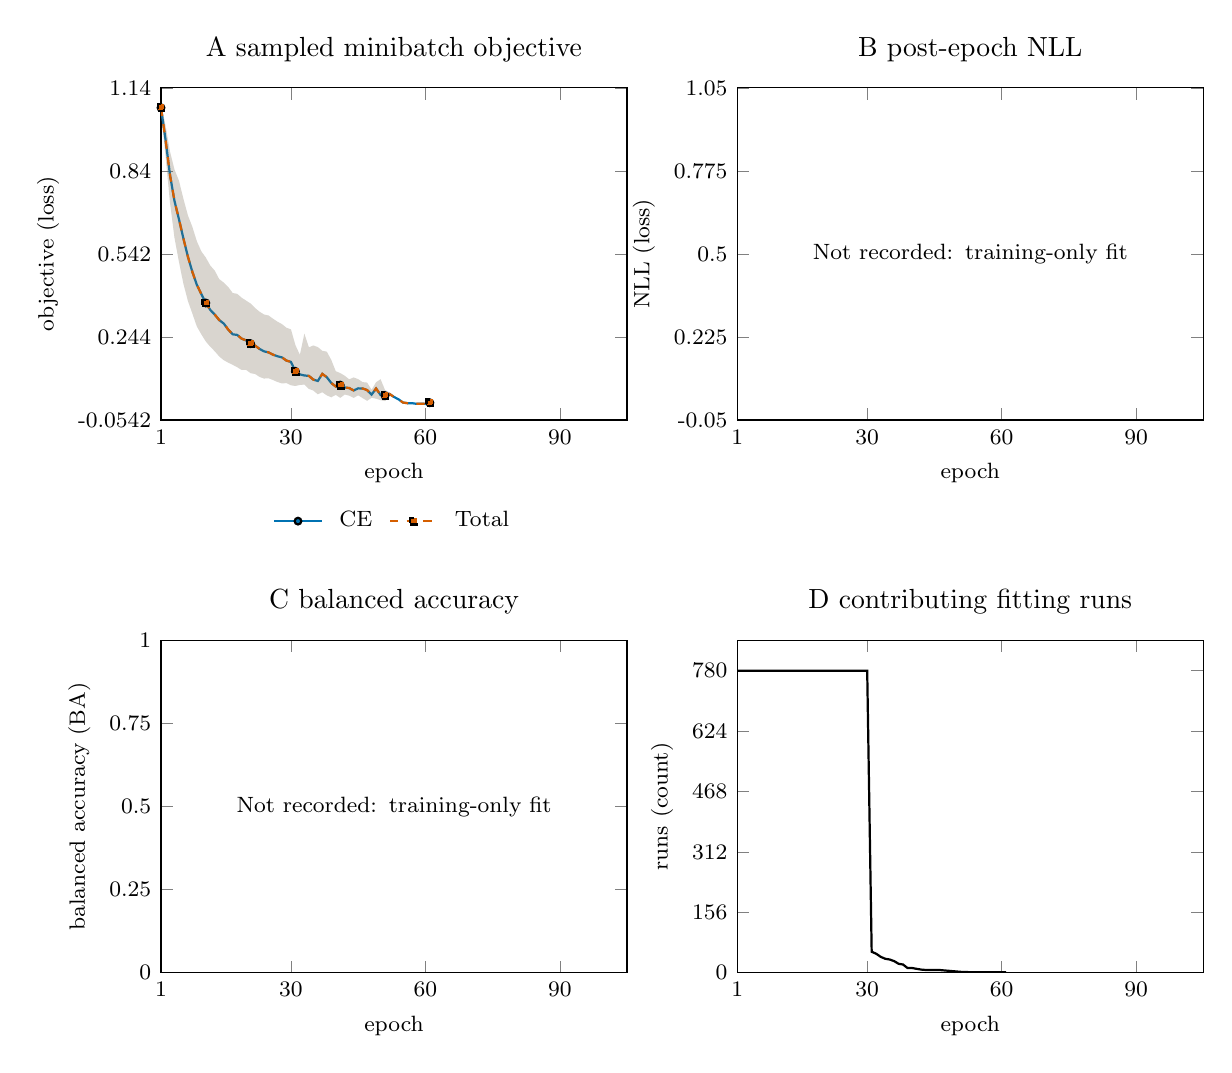
\begin{tikzpicture}
\begin{groupplot}[group style={group size=2 by 2, horizontal sep=14mm, vertical sep=28mm}]
\nextgroupplot[width=75mm, height=58mm, title={A sampled minibatch objective}, xlabel={epoch}, ylabel={objective (loss)}, xmin=1, xmax=105, xtick={1,30,60,90}, ymin=-0.05422497615218163, ymax=1.1387244991958141, ytick={-0.05422497615218163,0.24401239268481728,0.54224976152181625,0.84048713035881517,1.1387244991958141}, yticklabels={-0.0542,0.244,0.542,0.84,1.14}, tick label style={font=\fontsize{8}{9}\selectfont, text=black}, label style={font=\fontsize{8}{9}\selectfont, text=black}, title style={font=\fontsize{10}{11}\selectfont, text=black}, legend style={at={(0.5,-0.24)},anchor=north,draw=none,fill=none,font=\fontsize{8}{9}\selectfont,row sep=1pt,column sep=4pt,legend columns=2}]
\addplot[fill=oi-blue,opacity=0.15,draw=none,forget plot] coordinates {(1,1.0484078824520111) (2,0.89668757617473605) (3,0.72792637944221494) (4,0.60120482668280606) (5,0.51467146947979925) (6,0.43565788269042971) (7,0.374057836830616) (8,0.32829188369214535) (9,0.28190019205212591) (10,0.25375099331140516) (11,0.22798768281936646) (12,0.20893128067255021) (13,0.19271800257265567) (14,0.17401785012334586) (15,0.16083431411534549) (16,0.15194740258157252) (17,0.14414372704923153) (18,0.13554538488388063) (19,0.12555085318163037) (20,0.12580073326826097) (21,0.11401331117376685) (22,0.11113368552178145) (23,0.100631067994982) (24,0.09474580772221089) (25,0.095871465560048816) (26,0.089477245043963191) (27,0.082389031909406191) (28,0.07718879599124194) (29,0.07850692286156119) (30,0.07068762630224229) (31,0.06805370794609189) (32,0.071927586756646636) (33,0.07295701652765274) (34,0.057658925419673324) (35,0.051634450023993847) (36,0.038280232110992074) (37,0.045622431021183733) (38,0.034396330825984478) (39,0.027543608099222183) (40,0.036240720050409438) (41,0.025363278319127859) (42,0.03733051975432318) (43,0.033379607624374336) (44,0.025169695774093271) (45,0.034618109650909903) (46,0.024504842562600972) (47,0.014774615352507681) (48,0.02580781002761796) (49,0.022428777621826157) (50,0.017169004818424583) (51,0.013723403326002881) (52,0.034029080439358948) (53,0.028653693152591586) (54,0.020233712974004447) (55,0.0085620569880120456) (56,0.0063623774913139641) (57,0.0063939182437025011) (58,0.0039765757392160594) (59,0.0044916067272424698) (60,0.0037129376432858407) (61,0.0079071754880715162) (61,0.0079071754880715162) (60,0.0037129376432858407) (59,0.0044916067272424698) (58,0.0039765757392160594) (57,0.0063939182437025011) (56,0.0063623774913139641) (55,0.0085620569880120456) (54,0.020233712974004447) (53,0.028653693152591586) (52,0.04490472385659814) (51,0.05336170603404753) (50,0.092302412586286672) (49,0.081476864125579598) (48,0.054370098188519476) (47,0.080264954827725887) (46,0.082003450579941281) (45,0.09256108291447164) (44,0.098768152203410883) (43,0.091978191351518038) (42,0.10486001688987015) (41,0.11432684808969497) (40,0.12120560770854354) (39,0.16163126407191158) (38,0.19127765297889709) (37,0.19437089487910272) (36,0.20767334215342997) (35,0.21361494697630407) (34,0.20682391710579395) (33,0.25606092810630798) (32,0.18012007251381887) (31,0.21437640171498065) (30,0.27139084413647652) (29,0.27724470086395742) (28,0.29014191627502439) (27,0.29898765571415425) (26,0.30955650620162489) (25,0.32130529098212718) (24,0.32476068735122682) (23,0.33473324477672578) (22,0.34796781428158285) (21,0.36408180072903634) (20,0.37455628365278243) (19,0.38513757437467583) (18,0.39899059347808363) (17,0.40194735974073414) (16,0.42365082353353506) (15,0.43949427306652072) (14,0.4517033085227013) (13,0.48208577260375024) (12,0.50057888925075533) (11,0.52925987169146538) (10,0.55142734944820404) (9,0.58771480321884151) (8,0.6393095657229424) (7,0.68103928565979011) (6,0.74027076959609983) (5,0.80576295107603069) (4,0.84565715342760084) (3,0.9103191211819649) (2,1.0047352984547615) (1,1.0816313326358795)};
\addplot[color=oi-blue, mark=*, mark options={draw=black}, mark repeat=10, mark size=1.2pt, solid, line width=0.8pt] coordinates {(1,1.0676643848419189) (2,0.95488189160823822) (3,0.82688870280981064) (4,0.73329900950193405) (5,0.66755186021327972) (6,0.59805907309055328) (7,0.53269684687256813) (8,0.47778067737817764) (9,0.43151959776878357) (10,0.39835266023874283) (11,0.36611127480864525) (12,0.34117007628083229) (13,0.32446209900081158) (14,0.3046912532299757) (15,0.29243685305118561) (16,0.27066066674888134) (17,0.25371258333325386) (18,0.2514400165528059) (19,0.23818844370543957) (20,0.2316867969930172) (21,0.22013040818274021) (22,0.21314269118010998) (23,0.2010838259011507) (24,0.19238834735006094) (25,0.18876554444432259) (26,0.1805851086974144) (27,0.17476910911500454) (28,0.17066465970128775) (29,0.15923509653657675) (30,0.1545420060865581) (31,0.12055192748084664) (32,0.10961657855659723) (33,0.10586386919021606) (34,0.10428314562886953) (35,0.090888840146362782) (36,0.08613476762548089) (37,0.11144769843667746) (38,0.099613744765520096) (39,0.078870254452340305) (40,0.066098680021241307) (41,0.071254300884902477) (42,0.062614623922854662) (43,0.060675656422972679) (44,0.051972073502838612) (45,0.059578875079751015) (46,0.058973689912818372) (47,0.053450617007911205) (48,0.037217626580968499) (49,0.058890312095172703) (50,0.035719949984923005) (51,0.033542554680025205) (52,0.039466902147978544) (53,0.028653693152591586) (54,0.020233712974004447) (55,0.0085620569880120456) (56,0.0063623774913139641) (57,0.0063939182437025011) (58,0.0039765757392160594) (59,0.0044916067272424698) (60,0.0037129376432858407) (61,0.0079071754880715162)};
\addlegendentry{CE}
\addplot[fill=oi-vermillion,opacity=0.15,draw=none,forget plot] coordinates {(1,1.0484078824520111) (2,0.89668757617473605) (3,0.72792637944221494) (4,0.60120482668280606) (5,0.51467146947979925) (6,0.43565788269042971) (7,0.374057836830616) (8,0.32829188369214535) (9,0.28190019205212591) (10,0.25375099331140516) (11,0.22798768281936646) (12,0.20893128067255021) (13,0.19271800257265567) (14,0.17401785012334586) (15,0.16083431411534549) (16,0.15194740258157252) (17,0.14414372704923153) (18,0.13554538488388063) (19,0.12555085318163037) (20,0.12580073326826097) (21,0.11401331117376685) (22,0.11113368552178145) (23,0.100631067994982) (24,0.09474580772221089) (25,0.095871465560048816) (26,0.089477245043963191) (27,0.082389031909406191) (28,0.07718879599124194) (29,0.07850692286156119) (30,0.07068762630224229) (31,0.06805370794609189) (32,0.071927586756646636) (33,0.07295701652765274) (34,0.057658925419673324) (35,0.051634450023993847) (36,0.038280232110992074) (37,0.045622431021183733) (38,0.034396330825984478) (39,0.027543608099222183) (40,0.036240720050409438) (41,0.025363278319127859) (42,0.03733051975432318) (43,0.033379607624374336) (44,0.025169695774093271) (45,0.034618109650909903) (46,0.024504842562600972) (47,0.014774615352507681) (48,0.02580781002761796) (49,0.022428777621826157) (50,0.017169004818424583) (51,0.013723403326002881) (52,0.034029080439358948) (53,0.028653693152591586) (54,0.020233712974004447) (55,0.0085620569880120456) (56,0.0063623774913139641) (57,0.0063939182437025011) (58,0.0039765757392160594) (59,0.0044916067272424698) (60,0.0037129376432858407) (61,0.0079071754880715162) (61,0.0079071754880715162) (60,0.0037129376432858407) (59,0.0044916067272424698) (58,0.0039765757392160594) (57,0.0063939182437025011) (56,0.0063623774913139641) (55,0.0085620569880120456) (54,0.020233712974004447) (53,0.028653693152591586) (52,0.04490472385659814) (51,0.05336170603404753) (50,0.092302412586286672) (49,0.081476864125579598) (48,0.054370098188519476) (47,0.080264954827725887) (46,0.082003450579941281) (45,0.09256108291447164) (44,0.098768152203410883) (43,0.091978191351518038) (42,0.10486001688987015) (41,0.11432684808969497) (40,0.12120560770854354) (39,0.16163126407191158) (38,0.19127765297889709) (37,0.19437089487910272) (36,0.20767334215342997) (35,0.21361494697630407) (34,0.20682391710579395) (33,0.25606092810630798) (32,0.18012007251381887) (31,0.21437640171498065) (30,0.27139084413647652) (29,0.27724470086395742) (28,0.29014191627502439) (27,0.29898765571415425) (26,0.30955650620162489) (25,0.32130529098212718) (24,0.32476068735122682) (23,0.33473324477672578) (22,0.34796781428158285) (21,0.36408180072903634) (20,0.37455628365278243) (19,0.38513757437467583) (18,0.39899059347808363) (17,0.40194735974073414) (16,0.42365082353353506) (15,0.43949427306652072) (14,0.4517033085227013) (13,0.48208577260375024) (12,0.50057888925075533) (11,0.52925987169146538) (10,0.55142734944820404) (9,0.58771480321884151) (8,0.6393095657229424) (7,0.68103928565979011) (6,0.74027076959609983) (5,0.80576295107603069) (4,0.84565715342760084) (3,0.9103191211819649) (2,1.0047352984547615) (1,1.0816313326358795)};
\addplot[color=oi-vermillion, mark=square*, mark options={draw=black}, mark repeat=10, mark size=1.2pt, dashed, line width=0.8pt] coordinates {(1,1.0676643848419189) (2,0.95488189160823822) (3,0.82688870280981064) (4,0.73329900950193405) (5,0.66755186021327972) (6,0.59805907309055328) (7,0.53269684687256813) (8,0.47778067737817764) (9,0.43151959776878357) (10,0.39835266023874283) (11,0.36611127480864525) (12,0.34117007628083229) (13,0.32446209900081158) (14,0.3046912532299757) (15,0.29243685305118561) (16,0.27066066674888134) (17,0.25371258333325386) (18,0.2514400165528059) (19,0.23818844370543957) (20,0.2316867969930172) (21,0.22013040818274021) (22,0.21314269118010998) (23,0.2010838259011507) (24,0.19238834735006094) (25,0.18876554444432259) (26,0.1805851086974144) (27,0.17476910911500454) (28,0.17066465970128775) (29,0.15923509653657675) (30,0.1545420060865581) (31,0.12055192748084664) (32,0.10961657855659723) (33,0.10586386919021606) (34,0.10428314562886953) (35,0.090888840146362782) (36,0.08613476762548089) (37,0.11144769843667746) (38,0.099613744765520096) (39,0.078870254452340305) (40,0.066098680021241307) (41,0.071254300884902477) (42,0.062614623922854662) (43,0.060675656422972679) (44,0.051972073502838612) (45,0.059578875079751015) (46,0.058973689912818372) (47,0.053450617007911205) (48,0.037217626580968499) (49,0.058890312095172703) (50,0.035719949984923005) (51,0.033542554680025205) (52,0.039466902147978544) (53,0.028653693152591586) (54,0.020233712974004447) (55,0.0085620569880120456) (56,0.0063623774913139641) (57,0.0063939182437025011) (58,0.0039765757392160594) (59,0.0044916067272424698) (60,0.0037129376432858407) (61,0.0079071754880715162)};
\addlegendentry{Total}
\nextgroupplot[width=75mm, height=58mm, title={B post-epoch NLL}, xlabel={epoch}, ylabel={NLL (loss)}, xmin=1, xmax=105, xtick={1,30,60,90}, ymin=-0.050000000000000003, ymax=1.05, ytick={-0.050000000000000003,0.22500000000000003,0.5,0.77500000000000002,1.05}, yticklabels={-0.05,0.225,0.5,0.775,1.05}, tick label style={font=\fontsize{8}{9}\selectfont, text=black}, label style={font=\fontsize{8}{9}\selectfont, text=black}, title style={font=\fontsize{10}{11}\selectfont, text=black}]
\node[align=center, text width=55mm, font=\fontsize{8}{9}\selectfont] at (axis cs:53,0.5) {Not recorded: training-only fit};
\nextgroupplot[width=75mm, height=58mm, title={C balanced accuracy}, xlabel={epoch}, ylabel={balanced accuracy (BA)}, xmin=1, xmax=105, xtick={1,30,60,90}, ymin=0, ymax=1, ytick={0,0.25,0.5,0.75,1}, yticklabels={0,0.25,0.5,0.75,1}, tick label style={font=\fontsize{8}{9}\selectfont, text=black}, label style={font=\fontsize{8}{9}\selectfont, text=black}, title style={font=\fontsize{10}{11}\selectfont, text=black}]
\node[align=center, text width=55mm, font=\fontsize{8}{9}\selectfont] at (axis cs:53,0.5) {Not recorded: training-only fit};
\nextgroupplot[width=75mm, height=58mm, title={D contributing fitting runs}, xlabel={epoch}, ylabel={runs (count)}, xmin=1, xmax=105, xtick={1,30,60,90}, ymin=0, ymax=858.00000000000011, ytick={0,156,312,468,624,780}, yticklabels={0,156,312,468,624,780}, tick label style={font=\fontsize{8}{9}\selectfont, text=black}, label style={font=\fontsize{8}{9}\selectfont, text=black}, title style={font=\fontsize{10}{11}\selectfont, text=black}]
\addplot[color=oi-black, solid, line width=0.8pt] coordinates {(1,780) (2,780) (3,780) (4,780) (5,780) (6,780) (7,780) (8,780) (9,780) (10,780) (11,780) (12,780) (13,780) (14,780) (15,780) (16,780) (17,780) (18,780) (19,780) (20,780) (21,780) (22,780) (23,780) (24,780) (25,780) (26,780) (27,780) (28,780) (29,780) (30,780) (31,54) (32,49) (33,41) (34,36) (35,34) (36,30) (37,23) (38,21) (39,12) (40,12) (41,10) (42,8) (43,7) (44,7) (45,7) (46,7) (47,6) (48,5) (49,4) (50,3) (51,2) (52,2) (53,1) (54,1) (55,1) (56,1) (57,1) (58,1) (59,1) (60,1) (61,1)};
\end{groupplot}
\end{tikzpicture}
\par\vspace{6mm}
\begin{minipage}{175mm}
{\fontsize{8}{10}\selectfont RQ-S01 / Scope E: descriptive training diagnostics. 400-1800 cm-1 inputs: SG uses impulse replacement and Savitzky-Golay smoothing; arPLS uses impulse replacement and baseline correction; both finish with [0,1] min-max scaling. CE = chemical cross-entropy; SupCon = supervised contrastive; Paired = paired consistency; NLL = negative log-likelihood; BA = balanced accuracy. Authenticated complete monitor histories aggregated across unique fitting jobs into descriptive policy/recipe/stage curves. Curves summarize per-epoch minibatch-weighted training chemical cross-entropy and the composite total optimization objective; these sampled minibatch objectives differ from post-epoch evaluation negative log-likelihood. Auxiliary supcon/paired loss components are recipe-specific and are not directly comparable to the total objective across recipes. Validation metrics are recorded for source\_fit runs only and never substitute for a held-out test set; calibration\_model\_fit and final\_refit rows carry training-only diagnostics. Source\_fit optimization uses a 30-epoch minimum stopping threshold and a 200-epoch maximum; refit stages reuse the caller-selected duration. Curves are fitting-run-weighted descriptive summaries over correlated runs (seeds/splits). Lines show medians; 10th/90th percentiles describe variation among saved fitting runs, not confidence intervals. Only runs that reached each epoch contribute; early stopping changes the composition, and stopped runs are not carried forward. Fitting jobs are not independent chemical samples: the dataset has 598 spectra from 69 physical samples and 10 instruments. Coverage is limited to saved SG/arPLS monitor histories; historical MIN losses are not pooled or invented. A missing history is not a zero loss or proof of a failed model. These curves do not support hypothesis tests, superiority claims, model selection, or new uncertainty inference. P08 learned-method performance is reported elsewhere.}
\end{minipage}
\end{minipage}
\end{document}